\documentclass[12pt]{article}

\usepackage{graphicx}
\usepackage{amsmath}
\usepackage{amsfonts}
\usepackage{apacite}
\usepackage{natbib} 
\usepackage{url}
\usepackage[hidelinks]{hyperref}
\usepackage{cleveref}
\usepackage[utf8]{inputenc}
\usepackage{setspace}
\usepackage{caption}
\usepackage{verbatim}
\usepackage{placeins}
\usepackage{subfigure}
\usepackage{dsfont}
\usepackage{accents}
\usepackage{appendix} % For enhanced appendix formatting
\usepackage{todonotes}

\onehalfspacing

\newcommand{\jsh}[1]{\todo[inline,color=green!20, caption={2do}]{\textbf{Jack:}\\#1}}

\title{Insights into the prior to posterior transition through Wasserstein
distances and the power posterior}
\author{Damian Mingo, Jack S. Hale}
\date{\today}

\usepackage{glossaries}

\newacronym{wim}{WIM}{Wasserstein Impact Measure}  
\newacronym{nuts}{NUTS}{No-U-Turn sampler}  
\newacronym{swim}{sWIM}{prior scaled Wasserstein Impact Measure}  
\newacronym{bf}{BF}{Bayes factor}
\newacronym{mcmc}{MCMC}{Markov Chain Monte Carlo}
\newacronym{ott}{OTT}{Optimal Transport Tools}
\newacronym{tfp}{TFP}{Tensorflow Probability}


\begin{document}


\maketitle


\begin{abstract}

To ensure parameter estimates are robust to the specification of the prior it
is essential to check if different priors produce varying results. The recently
introduced Wasserstein Impact Measure measures the distance between two posteriors
induced

\end{abstract}

\section{Introduction}

\jsh{JSH TODO: Opening paragraph - similar to paper 2}

\jsh{JSH TODO: Narrow in on WIM. Measures distances between posteriors which are prior +
data (via likelihood). Explain what the WIM doesn't do.}

\jsh{JSH: TODO: Discuss new idea. Examine the continuous transition between prior and
posterior via the likelihood.}

Several measures of prior impact assessment have been developed. These measures
of prior impact are usually based on divergences such as the Kullback–Leibler
divergence or distances such as the Wasserstein distance. However, these
distances are not directly interpretable and cannot tell us the weight of the
impact of a prior distribution. We provide the weight of impact for prior
distributions relative to standard normal distributions.

Power posteriors have been used in many applications. One of such is the
calculation of the marginal likelihood \citep{friel2008marginal}. They are used
to calculate the objective \gls{bf} and are referred to there as fractional
posteriors \citep{ohaganPropertiesIntrinsicFractional1997}. They have been
applied to sample across multimodal distributions. We use the power posteriors
to understand how prior impacts posterior inference. For conjugate cases, we
derive and make use of analytic solutions. However, we use \gls{mcmc} to extend
our approach for models with no closed-form solution. In addition, we compute
the \gls{wim} of \cite{ghaderinezhadWassersteinImpactMeasure2022}, which
requires the calculation of Wasserstein distances. We use graphs to illustrate
the impacts of priors and how the priors transition to the posteriors.

\subsection{Contribution}

The main contributions of this paper are as follows. Using the concept of the
power posterior we construct a continuous family of posteriors between prior
and posterior by raising the usual likelihood to a power posterior constant
$\gamma \in [0, 1]$. To give a visual intuition of this transition, in
\cref{fig:skew_normal_powpos} we show posterior density plots of the power
posteriors living between a uniform prior the standard posterior for a
parameter describing the skewness of a dataset.

\jsh{JSH: Expand on last comment about plot}

\begin{figure}
\begin{center}
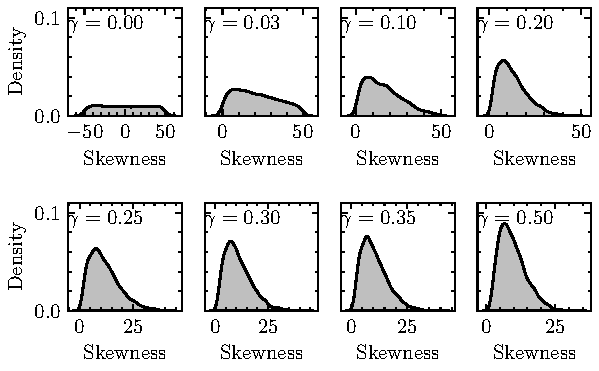
\includegraphics{imgs/uniform_pow.pdf}
\end{center}
\caption{Marginal posteriors for the skewness parameter show the transition
	from a uniform prior ($\gamma=0$) to various power posteriors
	($0 < \gamma \leq 0.5$). Posterior based on the frontier data set for the
	skew-normal distribution.}\label{fig:skew_normal_powpos}
\end{figure}

From the definition of the power posterior we derive extensions of three
standard conjugate results, namely the Normal-Normal, Normal-Inverse-Gamma and
Poisson-Gamma cases. These conjugate results show that for an observed data set
of size $n$ the product $\gamma n$ as the effective sample size of the observed
data, that is, $\gamma$ can be used to reduce the sample size of the data from
$n$ to $n\gamma$. An alternative intepretation, which can be seen by writing
the log-likelihood, is that $\gamma$ controls the relative weight of the
log-likelihood (and consequently the data) with respect to the log-prior.

With the definition of the power posterior in hand we then observe the
evolution of the Wasserstein distance between power posterior measures
$\mu_{\gamma}$ and the fixed prior measure $\mu_{0}$. These plots typically
show a sudden change in the Wasserstein distance as $\gamma$ is increased just
beyond zero (the prior is moved a large distance by a small effective sample
size of the data). As $\gamma$ is increased at some point the distance
`saturates' and increasing $\gamma$ further (i.e. increasing the effective
sample size) does not lead to the posterior moving significantly further away
from the prior. This saturation region gives us an indication of a saturation
sample size, that is, at which adding more data into the problem (implicitly
via the parameter $\gamma$) does not lead to an increase in the distance
between the power posterior and the prior.

\jsh{Finish this final paragraph}

In addition to looking at an prior to posterior transition for a single fixed
prior, we also look at the evolution of the Wasserstein distance under
different prior assumptions.

\section{Methodology}

\subsection{Power posterior}
We briefly recall the mathematical concept of the power posterior (sometimes
also called the fractional posterior) which is central to this paper. Let $y$
be some observed data and $p(y\, | \, \theta)$ be the likelihood function of a
model that depends on a set of parameters $\theta$ with associated prior
$p(\theta)$. Moreover, let $\gamma$ be an additional \emph{power posterior
constant} in the interval $[0, 1]$. Then the power posterior
\citep{friel2008marginal} can be defined as
\begin{equation}
\label{eq:pow_pos}
p(\theta \, | \, y,\gamma) := \frac{p(y \, | \, \theta)^\gamma p(\theta)}{z}, \quad \gamma \in [0, 1],
\end{equation}
where $z := p(y)$ is a normalising constant called the marginal likelihood. It
is straightforward to see that for $\gamma = 0$ we recover the usual Bayesian
prior $p(\theta)$ and for $\gamma = 1$ we recover the standard Bayesian
posterior $p(\theta \, | y)$. We emphasise that for intermediate values $\gamma
\in (0, 1)$ the resulting set of power posteriors forms a continuous
transition between the standard prior and posterior distribution.

\subsection{Wasserstein distance}
The definition of the $p$-Wasserstein distance ($W_p$) between two probability
measures $\mu, \nu$ defined on the spaces $\mathcal{X}$ and $\mathcal{Y}$ is 
\begin{equation}
W_p(\mu, \nu) = \inf_{\pi \in U(\mu, \nu)} \left(\int_{\mathcal{X} \times \mathcal{Y}}||x-y||^pd\pi(x, y) \right)^{1/p}, \quad p\geq 1,
\label{wasser:ana}
\end{equation}
where $U(\mu, \nu)$ is the set of joint probability measures on
$\mathcal{X}\times \mathcal{Y}$ \citep{villaniOptimalTransportOld2009}. The
Wasserstein distance has a natural intepreration as the minimum amount of work
required to reconfigure the mass of one distributoin into another. Calculating
the Wasserstein distance becomes non-trivial in moderate to high dimensions due
to the ill-posed nature of the squared Euclidean distance
\citep{cuturiMongeBregmanOccam2023}. 

\subsection{Posterior measures}
\jsh{Define all of the varios measures}

\subsection{Subsampling}
\jsh{Write definition of subsampling}

\subsection{Numerical methods}
We give a brief overview of the numerical methods used to generate the results.
For full details see the references provided below.

Samples from the power posteriors and priors are generated using \gls{mcmc},
specifically the \gls{nuts} \citep{hoffman2014}. We use the version implemented
within \gls{tfp} \citep{dillonTensorFlowDistributions2017} running on the JAX
backend \citep{jax2018github}.

We remark that exploring power posteriors within \gls{tfp} is straightforward
and only requires the programmatic definition of the log power-posterior. This
involves scaling the provided log-likelihood evaluation by $\gamma$ and then
adding the log-prior terms. This can be achieved in a few lines of code and the
resulting function passed to any of the \gls{mcmc} methods built-in to
\gls{tfp}.

The skew-normal distribution is not implemented in \gls{tfp}, so we wrote a
custom distribution using Distrax \citep{deepmind2020jax} following the
numerical methodology described in \citep{ghorbanzadeh_method_2014}. 

To calculate Wasserstein-1 distance for the one-dimensional problems we use the
Vallender formula \cite{vallender_calculation_1974} which relates the
1-Wasserstein distance between two probability measures $\mu_1$ and $\mu_2$ on
$\mathbb{R}$ with cumulative distribution functions $F_1(x)$ and $F_2(x)$,
respectively
\begin{equation}
W_1(\mu_1, \mu_2) = \int_{\mathbb{R}} | F_1(x) - F_2(x) | \; \mathrm{d}x.
\end{equation}
We approximate the Vallender formula using the dedicated function available in
SciPy \citep{2020SciPy-NMeth}. 

For the multi-dimensional case we cannot use to the Vallender formula to
compute the Wasserstein distance. Instead we use recent advances in
computational optimal transport to estimate the Wasserstein distance.
Specifically, we use entropic regularized optimal transport proposed in
\citep{NIPS2013_af21d0c9} and its implementation within the \gls{ott} library
\citep{cuturi2022optimal}. 


All code and data used to produce the results in this paper will be available
as supplementary material upon journal submission.

\section{Results}

\subsection{Normal-normal conjugate case with unknown mean}
Following standard arguments, it is possible to show that the distribution of
the power posterior for the following Bayesian model with dataset $x = (x_1,
\ldots, x_n)$
\begin{subequations}
\begin{align}
x_1, \ldots, x_n &\overset{\mathrm{iid}}{\sim} \mathcal{N}(m, \sigma^2), \\
m &\sim \mathcal{N}(m_0, \sigma_0^2),
\end{align}
\end{subequations}
is normally distributed
\begin{equation*}
m \;|\; x \sim \mathcal{N} \left( \left( \frac{1}{\sigma_0^2} + \frac{\gamma n}{\sigma^2} \right)^{-1} \left(\frac{m_0}{\sigma_0^2} + \frac{\gamma n \bar{x}}{\sigma^2}  \right), \left( \frac{1}{\sigma_0^2} + \frac{\gamma n}{\sigma^2} \right)^{-1} \right),
\end{equation*}
where $\bar{x} = (\sum x_i)/ n$ is the sample mean. We remark that, as
expected, the prior is recovered when $\gamma = 0$ and the classic
normal-normal with unknown mean conjugate result is recovered when $\gamma =
1$. The role of $\gamma$ in this context is to reduce the contribution of each
element of the dataset through the likelihood. More specifically for the
normal-normal case, the effective data set size is reduced from the standard
posterior ($\gamma = 1$) from $n$ to $n \gamma$ in the power posterior. Note
however, regardless of the value of $\gamma > 0$, the entire dataset $x$ is
still used in the update from prior to the power posterior.

The 2-Wasserstein metric ($p = 2$) for two non-degenerate normal
measures $\mu_1$ and $\mu_2$ on $\mathbb{R}$ with means $m_1, m_2 \in
\mathbb{R}$ and variances $\sigma_1^2, \sigma_2^2 \in \mathbb{R}_{>0} :=
\left\lbrace x \in \mathbb{R} \; | \; x > 0 \right\rbrace$, respectively, can
be found in closed form as
\begin{equation*}
W_{2} (\mu_1, \mu_2)^2 = \left( m_1 - m_2 \right)^2 + \sigma_1^2 + \sigma_2^2 - 2 \bigl( \sigma_2 \sigma_1^2 \sigma_2 \bigr)^{1/2}.
\end{equation*}
Consequently in this case there is no need to resort to approximate numerical
computations to compute the Wasserstein metric. In closed form the Wasserstein
metric between the prior measure $\mu_0$ and the measure induced by the power posterior
$\mu_\gamma$ is
\begin{equation*}
W_2(\mu_0, \mu_\gamma)^2 = \sigma_{0}^{2} + \frac{\sigma^{2} \sigma_{0}^{2}}{p} + \frac{\left(\gamma m_{0} n \sigma_{0}^{2} - \gamma n \sigma_{0}^{2} \bar{x}\right)^{2}}{p^{2}} - \frac{2 \sigma \sigma_{0}^{2}}{\sqrt{p}}
\end{equation*}
with $p = \gamma n \sigma_{0}^{2} + \sigma^{2}$ and the derivative of the
squared Wasserstein distance with respect to $\gamma$ given by
\tiny
\begin{equation*}
\frac{d}{d\gamma} [W_2(\mu_0, \mu_\gamma)^2] =
p^{-\frac{15}{2}}n \sigma_{0}^{2} \left(- p^{\frac{11}{2}} \sigma^{2} \sigma_{0}^{2} - 2 p^{\frac{9}{2}} \left(- \gamma n \sigma_{0}^{2} \bar{x} + m_{0} p - m_{0} \sigma^{2}\right) \left(- \gamma n \sigma_{0}^{2} \bar{x} - m_{0} \sigma^{2} + p \bar{x}\right) + p^{6} \sigma \sigma_{0}^{2}\right).
\end{equation*}
\normalsize
\jsh{Consider moving this to an appendix}
Letting $\gamma = 0$ it can be verified that $W_2(\mu_0, \mu_0)^2 = 0$, as
expected, and also that $\frac{d}{d\gamma}[W_2(\mu_0, \mu_0)^2] = 0$. 

In the first experiment we generate a (small) dataset of size $n = 10$ from a
normal distribution with zero mean and unit variance. We propose three prior
choices by adjusting the prior parameters $m_0$ and $\sigma_0^2$:
\begin{enumerate}
\item \emph{Non-informative prior}. $m_0 = 0$ and $\sigma_0^2 = 100$. With
this relatively flat prior we expect the posterior to be `data prominent'
and highly sensitive to the inclusion of information via the likelihood,
here controlled by the parameter $\gamma$.
\item \emph{Informative `correct' prior}. $m_0 = 0$ and $\sigma_0^2 = 2$.
This prior expresses definite information about the parameter that
coincidentally coincides with the true parameter. 
\item \emph{Informative `incorrect' prior}. $m_0 = -5$ and $\sigma_0^2 = 2$.
This prior expresses definite information about the parameter that
does not coincide with the true parameter value. 
\end{enumerate}
In \cref{fig:normal_normal_wasserstein_distance_different_priors} we calculate
the squared 2-Wasserstein distance between the posterior measure $\mu_\gamma$
for varying values of $\gamma$ and under the three prior assumptions just
described. All three distances appear to be monotonically increasing in
$\gamma$. The distance between the posterior and prior as $\gamma \to 1$ is
largest ($\sim10^2$) for the non-informative prior, and smallest ($\sim 1$) for
the informative `correct' prior. For the non-informative prior as $\gamma$ is
increased from $0$ we can see a very sudden increase in the metric, which
supports the intuition that the posterior is `data prominent' or `data
sensitive`. By comparison, the distance for the informative `correct' prior
evolves to its final distance more slowly, reflecting that the information
contained in the prior does not strongly disagree with that in the data. The
informative `incorrect' prior sits in between the two extreme cases.
\begin{figure}
\begin{center}
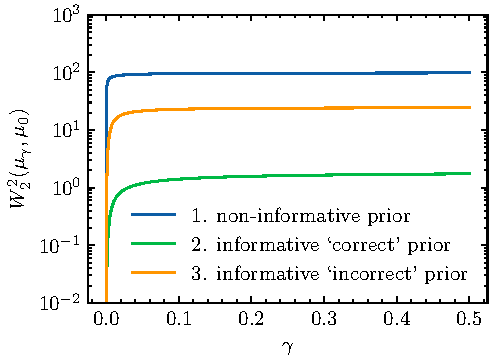
\includegraphics{imgs/normal_normal_wasserstein_distance_different_priors.pdf}
\end{center}
\caption{Normal-normal conjugate case; plot showing squared
2-Wasserstein metric between power posterior and prior against the
power posterior parameter $\gamma \in [0, \frac{1}{2}]$ under the three
different prior assumptions described in the text.}\label{fig:normal_normal_wasserstein_distance_different_priors}
\end{figure}

Given the intepretation of the parameter $\gamma n$ as an effective sample size
in the normal-normal setting, we briefly contrast the power posterior approach
with an approach based on using the standard posterior and varying the size $n$
of the dataset.

\jsh{JSH: To complete description of subsampling}

\FloatBarrier
\begin{figure}[ht!]
\begin{center}
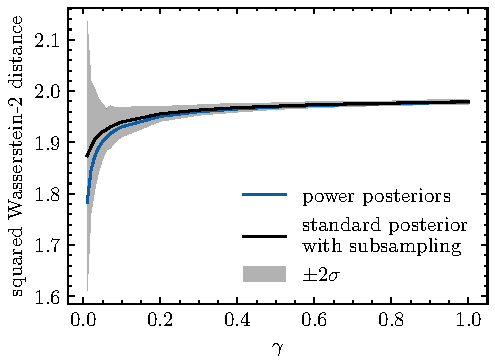
\includegraphics{imgs/gauss_knownsigma_subsample.pdf}
\end{center}
\caption{Normal-normal conjugate case with unknown mean. Wasserstein distance between the prior and power posteriors compared to the distance between the prior and standard posterior with subsampling. Both have the same mode and mean.}\label{fig:normal_normal_compare_with_subsampling}
\end{figure}

\subsection{Inverse-Gamma conjugate case with unknown variance}
Following standard arguments, it is possible to show that the distribution of
the power posterior for the following Bayesian model with dataset $x = (x_1,
\ldots, x_n)$
\begin{subequations}
\begin{align}
x_1, \ldots, x_n &\overset{\mathrm{iid}}{\sim} \mathcal{N}(m, \sigma^2), \\
\sigma^2 &\sim \text{Inv-Gamma}(\alpha, \beta)
\end{align}
\end{subequations}
with $\alpha, \beta \in \mathbb{R}_{>0}$, is distributed according to an
inverse gamma distribution
\begin{equation*}
\sigma^2 \; | \; x_1, \ldots, x_n \sim \text{Inv-Gamma}\left( \alpha + \frac{\gamma n}{2}, \beta + \frac{\gamma n}{2} s^2 \right). 
\end{equation*}
where $s^2 = (\sum_{i} \left( x_i - \mu \right)^2)/n$ is the uncorrected sample
variance. Again, setting $\gamma = 0$ recovers the prior, and setting $\gamma =
1$ recovers the usual conjugate result for the standard Bayesian posterior.


\FloatBarrier
\begin{figure}[ht!]
    \centering
    % First plot
    \subfigure[Data distribution compared to various power posteriors]{
        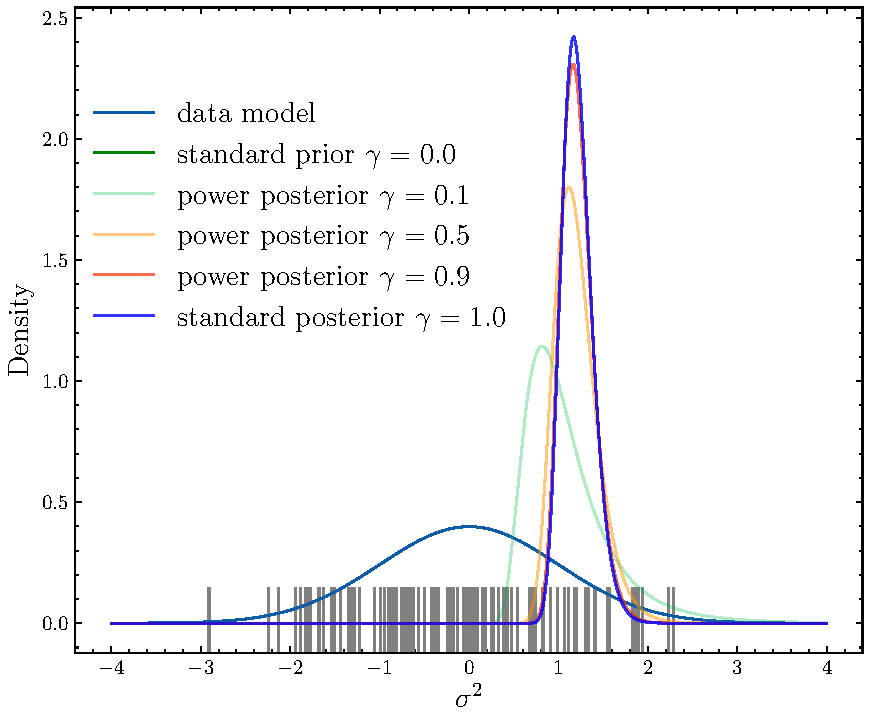
\includegraphics[width=0.45\textwidth]{imgs/data_posteriors_ivg.pdf} % Replace with your file name
        \label{fig:invg_dist}
    }
    \hfill % This ensures no extra space between the subfigures
    % Second plot
    \subfigure[Wasserstein distance between the standard prior and power posteriors for different distributions]{
        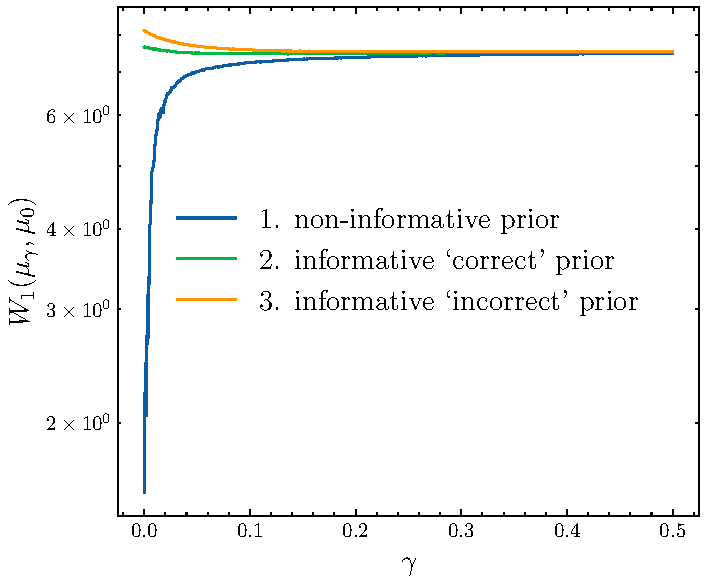
\includegraphics[width=0.45\textwidth]{imgs/wasserstein_distance_ivg.pdf} % Replace with your file name
        \label{fig:invg_wasser}
    }

    \caption{Comparison of power posteriors to the data model (a) and standard prior (b) for the inverse gamma conjugate case.}
    \label{fig:ing_conju}
\end{figure}
\jsh{I cannot distinguish between the two blues}

\subsection{Poisson-Gamma conjugate case with unknown rate}
\jsh{There is no description or analysis of these experiments - what are the
parameters of the priors? How big is the dataset?}

The distribution of the power posterior of the following Bayesian model with
dataset $x = (x_1, \ldots, x_n)$ 
\begin{subequations}
\begin{align}
x_1, \ldots, x_n &\overset{\mathrm{iid}}{\sim} \text{Poisson}(\lambda), \\
\lambda &\sim \text{Gamma}(\alpha, \beta),
\end{align}
\end{subequations}
where $\lambda \in \mathbb{R}_{>0}$ is the unknown rate parameter, and $\alpha,
\beta \in \mathbb{R}_{>0}$ are prior parameters is given by
\begin{equation}
\lambda \; | \; x \sim \text{Gamma} \left( \alpha + \gamma n \bar{x}, \beta + \gamma n \right)
\end{equation}



\begin{figure}[htbp]
    \centering
    % First plot
    \subfigure[Standard prior compared to various power posteriors]{
        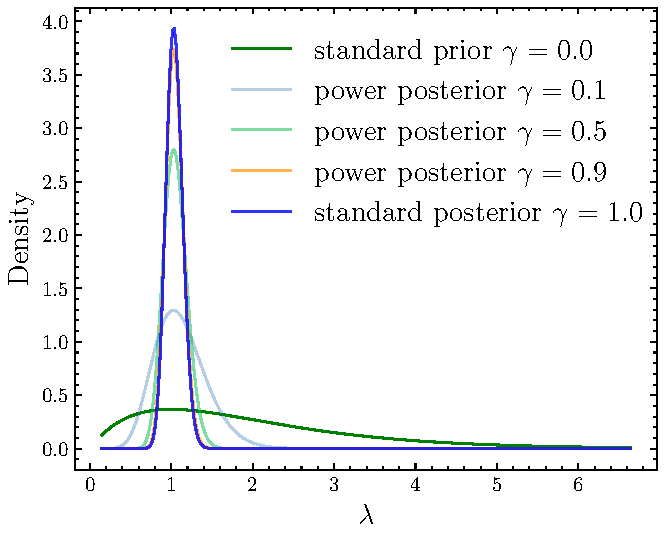
\includegraphics[width=0.45\textwidth]{imgs/data_posteriors_gamma.pdf} % Replace with your file name
        \label{fig:pois_gamma}
    }
    \hfill % This ensures no extra space between the subfigures
    \subfigure[Wasserstein distance between the power posteriors and standard prior up to $\gamma=0.5$]
{
        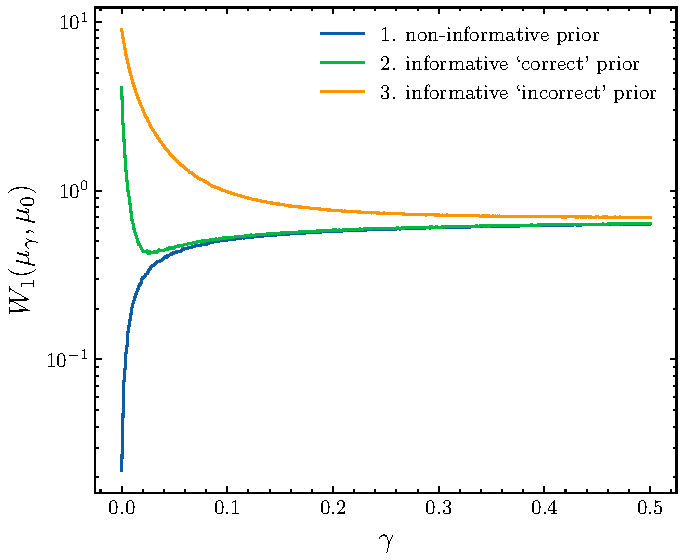
\includegraphics[width=0.45\textwidth]{imgs/wasserstein_distance_gamma.pdf} % Replace with your file name
        \label{fig:pois_gama_was}
    }

    \caption{Poisson-Gamma conjugate case with unknown rate}
    \label{fig:poisson_ga_conju}
\end{figure}
\jsh{Plots are too small}

\begin{figure}
\begin{center}
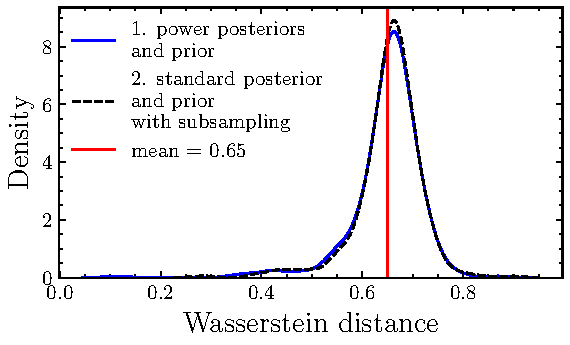
\includegraphics{imgs/poisson_gamma_subsample.pdf}
\end{center}
\caption{Distribution of the Wasserstein distance between the prior and the
	standard posterior ($\gamma=1.0$) with subsampling of the data and
	distribution of the Wasserstein distance between the power posteriors
	and priors. Both distributions very close with a mean of 0.65. Poisson
	Gamma case conjugate case.}\label{fig:poisson_gamma_sub}
\end{figure}
\jsh{I do not understand how the Wasserstein distance between the power
posterior and prior can be a random variable (and hence be plotted as a
distribution). The calculation is 'deterministic' if the prior and power
posterior chains are well converged.}
\jsh{I don't see the necessity of 'and prior' in the legend.}
\jsh{Text of x and y labels is crazy large, also on other plots}

\begin{comment}
\begin{figure}[htbp]
  \centering
  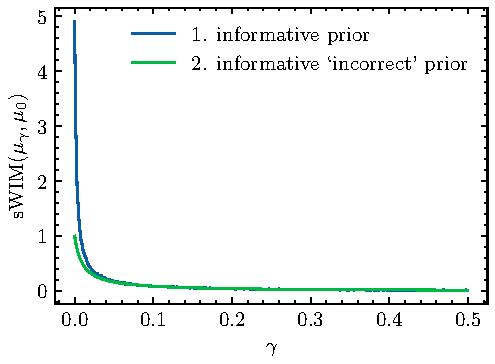
\includegraphics{imgs/swim_poisson_gamma_con.pdf} 
  \caption{Poisson-Gamma conjugate case with unknown rate; Plot showing the
	prior scale WIM between power posteriors with a non-informative prior
	as baseline against the power posterior parameter $\gamma \in [0,
	\frac{1}{2}]$. The sWIM value of 0.40 seems to be the elbow point where
	the plots levels off, similar to the scree plot in Principal component
	analysis.} 
  \label{fig:swim_poisson_ga} 
\end{figure}
\end{comment}
\jsh{Which prior?}


\subsection{Skew-normal distribution}
To gain more insight into prior impacts, we analysed the frontiers data set
found in the R package sn \citep{azzalini2023}. This data set has been analysed
by \cite{ghaderinezhadWassersteinImpactMeasure2022}. The data set is
interesting because the maximum likelihood estimate is unrealistic. The data is
generated by drawing 50 samples from a skew-normal distribution with a skewness
parameter of 5. The density of a random variable $x$ that follows a skew normal
distribution \citep{azzaliniClassD1985} is in \cref{skew_n}. Where $\phi$ is
the standard normal probability density function, $\Phi$ is the cumulative
distribution function of the standard normal distribution, $\mu$ is the
location, $\sigma$ is the scale parameter and $\alpha$ is the skewness
parameter.
\begin{equation}
    f(x; \alpha) = \frac{2}{\sigma} \phi \left( \frac{x - \mu}{\sigma} \right) \Phi \left( \alpha \frac{(x - \mu)}{\sigma}  \right), \quad x \in \mathbb{R}
    \label{skew_n}
\end{equation}
\jsh{You should not use the reference functionality to introduce an equation
directly next to its definition. Place definitions of parameters afterwards
(see Christophe's paper)}

We fit the skew-normal distribution to the data with different sets of priors
for the skewness parameter as in
\cite{ghaderinezhadWassersteinImpactMeasure2022}. We compare the Wasserstein
distance between various power posteriors and the prior. The priors are:
\begin{itemize}
\item Uniform prior
\item Jeffreys prior
\item Bayes-Laplace prior
\item Beta total variation prior (BTV)
\item Normal prior
\end{itemize}
\jsh{Seems unnecessary to use an explicit list incorporate into a sentence.}
The squared Wasserstein distance between the priors and the power posteriors
are in \cref{fig:skew_diff_priors}. The results suggest the difference between
the Uniform and the Jeffrys priors is very small. However, the distance between
the prior ($\gamma=0$) and the power posteriors increases with an increase in
$\gamma$ but becomes stable as $\gamma$ approaches 1. These insights are more
noticeable in the \gls{swim} compared to the squared Wasserstein distances.
\jsh{This plot is huge, please make it smaller}.
\begin{figure}
\begin{center}
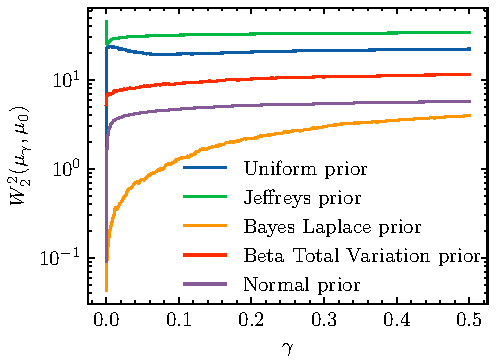
\includegraphics{imgs/wasser_distskew.pdf}
\end{center}
\caption{Squared Wasserstein distance between the prior and various power
posteriors for different values $\gamma \in [0, 0.5]$ on the frontiers
data set.}\label{fig:skew_diff_priors}
\end{figure}
\jsh{Plot too big. No intepretation/discussion of result in figure caption.}
\jsh{I would remove this stuff on sWIM entirely as discussed.}
Hence, we also explore the concept of \gls{swim} introduced in ODE paper. We
use Jeffrys prior and the Uniform prior as baseline priors for this. The
results are in plots \cref{fig:swimdistskew}. We can observe that the
\gls{swim} drops to zero as the prior transitions to the posterior. That is, as
$\gamma$ increases from 0 to 0.5. When the Jeffreys prior is used as the
baseline, the \gls{swim}  drops from 2.0 (\cref{fig:swimdistskew} A) to near
zero. When the baseline is a uniform uniform prior, the \gls{swim} drops from
1.0 to closer to 0.2. Hence, one can infer that the \gls{swim} is closer to
zero when there is no impact compared to a baseline prior. Also, the \gls{swim}
is closer to or greater than 1.0 when the prior impact is different from the
baseline prior. When the baseline prior is noninformative, a \gls{swim} value
close to zero indicates the prior in question is noninformative. This is seen
in (\cref{fig:swimdistskew} A), where the dashed line seems to have a constant
slope very close to zero for all values of $\gamma$. The inset shows the
\gls{swim} values are very close to zero. When the baseline is a uniform
distribution, the \gls{swim} are below one but have a minimum value of 0.2,
which is further from zero compared to when the baseline is Jefferys prior. The
fact that the \gls{swim} for the Uniform and the Jeffreys prior is close to
zero, as shown by the dashed line in \cref{fig:swimdistskew}A, confirms that
these two priors are closest. Another interesting visual is the density plot of
the priors and the power posteriors. Plots of the two closest priors, the
Uniform and Jeffreys priors, illustrate how the prior density transitions to
the posterior. For the Uniform prior, the mode is not visible, but as $\gamma$
starts increasing, a mode becomes visible, and the Uniform distribution starts
transitioning into a skew distribution. On the other hand, the mode is visible
for Jeffreys prior, but there is no skewness. As $\gamma$ increases, the mode
becomes more visible, and skewness becomes visible. As the value of $\gamma$
increases, the mode becomes more peaked, and the range of the skewness
parameter decreases.


\begin{figure}
\begin{center}
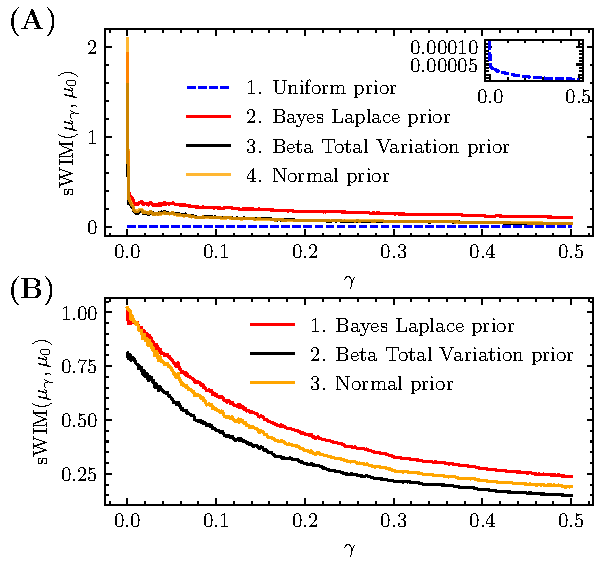
\includegraphics{imgs/swim_distskew.pdf}
\end{center}
\caption{Prior scale WIM for the skewness parameter of the skew normal
	distribution with \textbf{(A)} Jeffrys prior as the baseline prior and
	\textbf{(B)} the uniform prior as the baseline prior. For (A), 0.40 is
	the sWIM value at which the elbow levels off similar to principal
	component analysis.}\label{fig:swimdistskew}
\end{figure}
\jsh{I do not understand what is plotted here - the sWIM is defined between
posterior measures, not posterior and prior measures}

\begin{figure}
\begin{center}
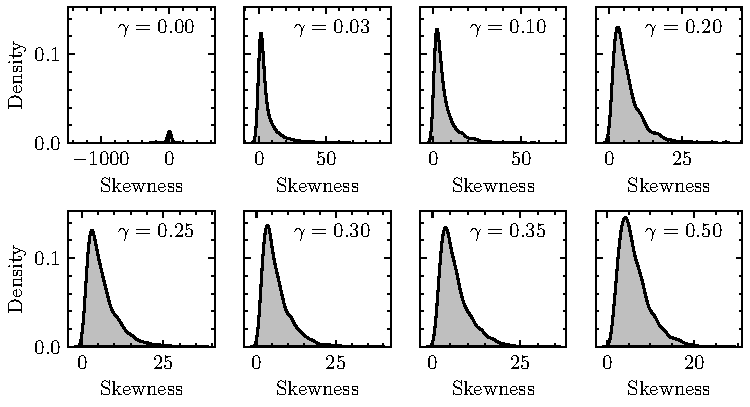
\includegraphics{imgs/Jeffreys.pdf}
\end{center}
\caption{Marginal posteriors for the skewness parameter show the transition
	from Jeffreys prior ($\gamma=0$) to various power posteriors
	($0<\gamma\leq1$).  Posterior based on the frontier data set for the
	skew-normal distribution. }\label{fig:skew_jeff_powpos}
\end{figure}

\clearpage
\begin{comment}
\subsection{Simple linear regression}

\begin{subequations}
\begin{align}
        Y|\beta_0, \beta_1,  \epsilon  &\sim \mathcal{N} (\beta_0 + \beta_1 X_1,  \epsilon)\\
    \beta_0  &\sim \mathcal{N}(0.0, 10.0)\\
     \beta_1  &\sim \mathcal{N}(0.0, 10.0)\\
     \epsilon & \sim \text{IG}(1.0, 0.5)
\end{align}
\end{subequations}

\begin{figure}[h]
\begin{center}
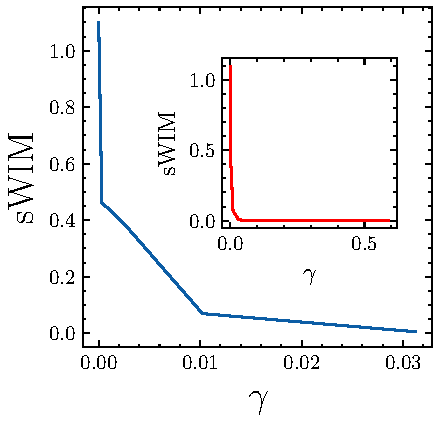
\includegraphics{imgs/swimgamma.pdf}
\caption{There is a sharp change in the sWIM closer to 0.40. This is similar to the previous examples when the elbow level off close to 0.40. }
\end{center}
\end{figure}

\begin{figure}[h]
\begin{center}
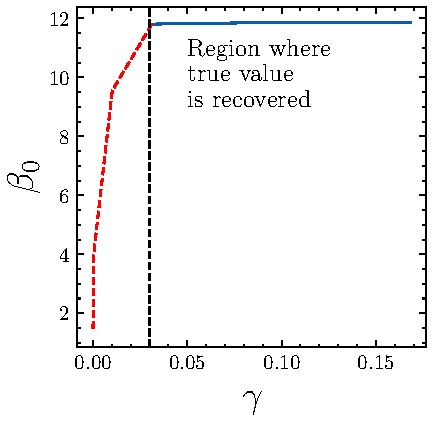
\includegraphics{imgs/betagamma.pdf}
\end{center}
\end{figure}
\end{comment}
\section{Conclusion}
\clearpage
\begin{appendices}
\jsh{These appendices are not referenced in the main text}
\section{Normal-normal conjugate case with unknown mean}
\subsection{Standard posteriors,  $\gamma = 1$.}
\jsh{All cases: Once you have the derivations for the standard result which do
not need to be repeated, these are three or four line proofs.}
\jsh{Use ams theorem environment}
\jsh{There is no statement of what you will prove, or definitions of any of the terms}
\jsh{There is no explanation or text to explain these derivations. This is a totally standard result and should just be repeated 'as a matter of fact'.}
\jsh{Aren't the likelihood and prior specified?}
\jsh{You cannot split equations across the result and its proof}
\begin{equation*}
\begin{aligned}
    x_i &|\mu\sim \mathcal{N}(\mu,\sigma^2),\quad \bar{x}= \frac{(\Sigma x_i)}{n}\\
    &\implies \bar{x}|\mu \sim \mathcal{N}(\mu,\sigma^2)\\
    p(x_1,\ldots,x_n|\mu)&\propto \frac{1}{\sigma}\exp\left(-\frac{1}{2\sigma^2}\sum(x_i-\mu)^2\right)\\
    \text{Proof}\\
    &\propto \exp\left(-\frac{1}{2\sigma^2}\sum(x_i^2-2x_i\mu +n\mu^2)\right)\\
    &\propto \exp\left(-\frac{n}{2\sigma^2}(-2\bar{x}\mu + \mu^2)\right)\\
     &\propto \exp\left(-\frac{n}{2\sigma^2}(\bar{x} - \mu)^2\right)\\
     &\propto p(\bar{x}, \mu)\\
\text{Likelihood} \\
    x_i &|\mu\sim \mathcal{N}(\mu,\sigma^2)\\
\text{Prior}\\
\mu &\sim \mathcal{N}(\mu_0,\sigma^2_0)
    \end{aligned}
\end{equation*}
\begin{equation*}
\begin{aligned}
(Z_1, Z_2) &\sim \mathcal{N}_2 \left(\mu, \Sigma \right)\\
    E(Z_1 | Z_2) &= E(Z_1) + \frac{\text{Cov}(Z_1, Z_2)}{\text{Var}(Z_2)} \left( Z_2 - E(Z_2) \right) \\
    \text{Var}(Z_1 | Z_2) &= \text{Var}(Z_1) - \frac{\text{Cov}(Z_1, Z_2)}{\text{Var}(Z_2)}\\
   x &\rightarrow Z_2 \quad \mu \rightarrow Z_1\\
   x&= \mu+\sigma\epsilon \quad \epsilon \sim N(0,1)\\
   \mu &= \mu_0 + \sigma\delta \quad \delta \sim N(0, 1)\\
   E(x) &= \mu_0\\
   & \text{Var}(x) = E[\text{Var}(x \mid \mu)] + \text{Var}[E(x \mid \mu)] \\
   & \quad = E[\sigma^2] + \text{var}(\mu) \\
   & \quad = \sigma^2 + \sigma_0^2.\\
    \text{Cov}(x, \mu) &= E[(x - \mu_0)(\mu - \mu_0)] \\
    &= E[x\mu - \mu_0 \mu - \mu_0 x + \mu_0^2] \\
    &= E[x\mu - \mu_0^2 - \mu_0 x + \mu_0^2] \\
    &= \sigma^2 \\
    E(\mu \mid x) &= \mu_0 + \frac{\sigma_0^2}{\sigma^2 + \sigma_0^2}(x - \mu_0) \\
    \text{Var}(\mu \mid x) &= \frac{\sigma^2 \sigma_0^2}{\sigma^2 + \sigma_0^2} \\
    &= \left( \frac{1}{\sigma_0^2} + \frac{1}{\sigma^2} \right)^{-1} \\
    &= (\tau_0 + \tau)^{-1}\\
    E(\mu \mid \bar{x}) &= \mu_0 + \frac{\sigma^2}{\sigma^2 + \sigma_0^2}(\bar{x} - \mu_0)
\end{aligned}
\end{equation*}

\subsection{Power posteriors, $\gamma \in [0,1]$.}
\jsh{Third equation is incorrect}
\begin{equation*}
\begin{aligned}
  p(x|\mu)^\gamma&\propto \frac{1}{\sigma}\exp\left(-\frac{1}{2\sigma^2}(x_i-\mu)^2\right)^\gamma\\
    (e^m)^\gamma &= e^{\gamma\relax m}, \quad (ae^m)^\gamma = a^{\gamma}e^{m\gamma}\\
p(x|\mu)^\gamma&\propto \frac{1}{\sigma\gamma}\exp\left(-\frac{\gamma}{2\sigma^2}(x-\mu)^2\right)\\
 x &|\mu \sim \mathcal{N}\left(\mu,\frac{\sigma^2}{\gamma}\right)\\
\bar{x} &|\mu \sim \mathcal{N}\left(\mu,\frac{\sigma^2}{\gamma\relax n}\right)\\
    E(\mu \mid \bar{x}) &= \mu_0 + \frac{\sigma_0^2}{\frac{\sigma^2}{\gamma \relax n} + \sigma_0^2}(\bar{x} - \mu_0) \\ 
    \text{Var}(\mu \mid \bar{x})&= \left( \frac{1}{\sigma_0^2} + \frac{\gamma\relax n}{\sigma^2} \right)^{-1} \\
       E(\mu \mid \bar{x}) &= \frac{1}{\frac{1}{\sigma_0^2} + \frac{\gamma n}{\sigma^2}} 
    + \left( \frac{\mu_0}{\sigma_0^2} + \frac{\gamma n \bar{x}}{\sigma^2} \right)\\
    \text{Var}(\mu \mid \bar{x})&= \left( \frac{1}{\sigma_0^2} + \frac{\gamma\relax n}{\sigma^2} \right)^{-1} \\
    \end{aligned}
\end{equation*}
\begin{equation}
\mu \;|\; x \sim \mathcal{N} \left( \left( \frac{1}{\sigma_0^2} + \frac{\gamma n}{\sigma^2} \right)^{-1} \left(\frac{\mu_0}{\sigma_0^2} + \frac{\gamma n \bar{x}}{\sigma^2}  \right), \left( \frac{1}{\sigma_0^2} + \frac{\gamma n}{\sigma^2} \right)^{-1} \right)
\end{equation}

\section{Inverse-Gamma conjugate case with unknown variance}
\jsh{These results are all standard and can just be summarised}
\subsection{Standard posterior  $\gamma = 1$.}
\begin{equation*}
\begin{aligned}
    p(x, \alpha,\beta) &= \frac{\beta^\alpha}{\Gamma(\alpha)} (x^2)^{-\alpha - 1} \exp\left(-\frac{\beta}{x}\right)\\
p(x|\sigma^2) &= \frac{1}{\sigma} \exp\left(-\frac{1}{2\sigma^2} (x - \mu)^2 \right)
    \end{aligned}
\end{equation*}

\textbf{Combine prior and likelihood}\\
\jsh{Again, these results are standard so you can just repeat them, then explain the reasoning/logic behind the power posterior}
\begin{equation*}
\begin{aligned}
p(\sigma^2 | \alpha, \beta) &\propto p(x|\sigma^2) p(\sigma^2| \alpha,\beta)\\
&=\frac{\beta^\alpha}{\Gamma(\alpha)} (\sigma^2)^{-\alpha - 1} \exp\left(-\frac{\beta}{\sigma^2}\right) \frac{1}{\sigma} \exp\left(-\frac{1}{2\sigma^2} (x - \mu)^2 \right)\\
&=\frac{\beta^\alpha}{\Gamma(\alpha)} (\sigma^2)^{-\alpha - 1}(\sigma^2)^{-\frac{1}{2}} \exp\left(-\frac{\beta+\frac{1}{2}(x-\mu)^2}{\sigma^2}\right)\\
&=\frac{\beta^\alpha}{\Gamma(\alpha)} (\sigma^2)^{\alpha +\frac{1}{2} -1}\exp\left(-\frac{\beta+\frac{1}{2}(x-\mu)^2}{\sigma^2}\right)\\
&\propto (\sigma^2)^{-\alpha +\frac{1}{2}-1}\exp\left(-\frac{\beta+\frac{1}{2}(x-\mu)^2}{\sigma^2}\right) \\
\sigma^2 | x &\sim \text{IG}\left(\alpha + \frac{1}{2}, \beta + \frac{1}{2} (x - \mu)^2 \right)
\end{aligned}
\end{equation*}

\textbf{Extension to multiple measurements}
\begin{equation*}
    \sigma^2 | x_1, \ldots, x_n \sim \text{IG}\left(\alpha + \frac{n}{2}, \beta + \frac{1}{2} \sum(x_i - \mu)^2 \right)
\end{equation*}

\begin{equation*}
    \begin{aligned}
        p(x_1, \ldots, x_n|\sigma^2 )= (2\pi)^{-\frac{k}{2}}\det\left(\Sigma\right)^{-\frac{1}{2}}\exp\left(-\frac{1}{2}(x-\mu)^T\Sigma^{-1}(x-\mu)\right)
    \end{aligned}
\end{equation*}
\[\Sigma=\sigma^2I\]



\begin{equation*}
    \sigma^2 \mid x_1, \ldots, x_n \sim \text{IG}\left(\alpha + \frac{n}{2}, \beta + \frac{1}{2} \sum (x_i - \mu)^2 \right)
\end{equation*}

\begin{equation*}
    \begin{aligned}
        p(x_1, \ldots, x_n \mid \sigma^2) &= (2\pi)^{-\frac{k}{2}} \det(\Sigma)^{-\frac{1}{2}} \exp\left(-\frac{1}{2}(\underaccent{\tilde}{x} - \underaccent{\tilde}\mu)^T \Sigma^{-1} (\underaccent{\tilde}x - \underaccent{\tilde}\mu)\right)\\
        \underaccent{=}\Sigma &= \sigma^2 I
    \end{aligned}
\end{equation*}

\begin{equation*}
    \begin{aligned}
    \underaccent{=}\Sigma&=\det(\sigma^2\underaccent{=}I)(\sigma^2)^n1\\
    &\propto(\sigma^{2n})^{-\frac{1}{2}}\exp\left(\frac{1}{2\sigma^2}\sum(x_i-\mu)^2\right)\\
    &\propto(\sigma^{2})^{-\frac{n}{2}}\exp\left(\frac{1}{2\sigma^2}\sum(x_i-\mu)^2\right)
 \end{aligned}
\end{equation*}

\subsection{Power posteriors, $\gamma \in [0,1]$.}
\begin{equation}
    \begin{aligned}
        [p(x_1, \ldots, x_n \mid \sigma^2)]^\gamma &=(\sigma^{2})^{-\frac{\gamma n}{2}}\exp\left(-\frac{\gamma}{2\sigma^2}\sum(x_i-\mu)^2\right)\\
        \sigma^2 &| x_1, \ldots, x_n \sim \text{IG}\left(\alpha+ \frac{\gamma n}{2}, \beta+\frac{\gamma}{2}\sum(x_i -\mu)^2\right)
    \end{aligned}
\end{equation}
\end{appendices}
\section{Poisson-Gamma conjugate case with unknown rate}
\subsection{Standard posterior $\gamma=1$.}
\begin{equation*}
    \begin{aligned}
        P(x \mid \lambda) &= Pr(x=k)\\
 &=\frac{\lambda^ke^{-\lambda}}{k!}
    \end{aligned}
\end{equation*}

\textbf{Multiple measurements}
\begin{equation*}
    \begin{aligned}
        P(\underaccent{\tilde}x \mid \lambda) &= \prod_{i=1}^n \frac{\lambda^{x_i} e^{-\lambda}}{x_i!}\\
        &= \frac{e^{-n \lambda}\lambda^{\sum x_i}}{\prod_{i=1}^n (x_i!)}
    \end{aligned}
\end{equation*}
\subsection{Power posteriors, $\gamma \in [0,1]$.}
\begin{equation*}
    \begin{aligned}
[P(\underaccent{\tilde}x \mid \lambda)]^\gamma &=  \frac{e^{-n \gamma\lambda}\lambda^{\gamma\sum x_i}}{\prod_{i=1}^n (x_i!)\gamma}\\
         p(\lambda) &= \frac{\beta^\alpha}{\Gamma(\alpha)} \lambda^{\alpha-1} e^{-\beta \lambda},\quad \lambda >0\\
          P(\underaccent{\tilde}x \mid \lambda)  p(\lambda)&= \lambda^{\sum x_i + \alpha - 1} e^{-(n\lambda + \beta\lambda)} \frac{\beta^\alpha}{\Gamma(\alpha)}\\
    \end{aligned}
\end{equation*}

\jsh{Remove under accent tildes, not necessary}
\begin{equation}
    \lambda|\underaccent{\tilde}x \sim \text{Gamma}\left(\gamma\sum x_i+\alpha, \gamma n+\beta\right)
\end{equation}

\bibliographystyle{apacite}
\bibliography{ref}

\end{document}
